\begin{abstract}
Release engineers need to identify failed coding-agent tasks before integrating their patches. We study task-end screening of 284 public SWE-agent trajectories using local, frozen MiniLM log embeddings and CodeBERT patch embeddings. A normal-reference nearest-neighbor detector reaches only 0.481 balanced accuracy in five-fold exploratory evaluation, flagging 14 of 54 successes while missing 179 of 230 failures. An inductive empirical-tail numeric control reaches 0.657 balanced accuracy, and supervised character TF-IDF reaches 0.652. Controlled comparisons show that patch-only embeddings outperform equal-weight log--patch fusion; reference contamination has small, nonmonotonic effects. We report raw confusion matrices, paired conditional uncertainty intervals, and traceable errors. No evaluated method meets our joint recall, false-alarm, and unflagged-success targets. More text information alone does not establish a reliable release gate, and failure prevalence of 81\% limits the classical rare-anomaly interpretation.
\end{abstract}

\section{Introduction}
Coding agents produce commands, observations, and patches, but a completed run need not resolve its issue \citep{yang2024sweagent}. Our stakeholder is a release engineer deciding which completed runs deserve extra inspection before integration. An alert requests review; absence of an alert does not authorize release.

Our application is \textbf{Category 4: Text / Logs}. Commands mix natural language, source code, tracebacks and repository conventions. Compressing them to counts loses content, but a general embedding may capture similarity rather than correctness. We ask: \emph{Can local text/code representations improve failure screening over numeric workflow features under a common false-alarm calibration policy?}

Normal means officially resolved; failure means officially unresolved. Successful \texttt{django-13230} is falsely flagged by our detector, whereas failed \texttt{sympy-12454} is close to successful reference vectors and escapes. These labels do not establish deception, reward hacking or false completion claims. Our contributions are a shared-partition NLP/numeric comparison, controlled representation/channel/contamination studies, and traceable confusion/error analyses that expose the limits of the resulting detector.

\section{Related Work}
SWE-bench \citep{jimenez2024swebench} evaluates patches on 2,294 GitHub issues from 12 Python repositories; its original best model resolves 1.96\%. SWE-agent \citep{yang2024sweagent} introduces an agent-computer interface and reports 12.5\% pass@1 on full SWE-bench and 87.7\% on HumanEvalFix. These are issue-solving results, not directly comparable to screening metrics.

Sentence-BERT \citep{reimers2019sentencebert} learns sentence representations for semantic comparison. We use the public MiniLM checkpoint with explicit chunk/token pooling, without fine-tuning. CodeBERT \citep{feng2020codebert} pretrains on programming and natural languages; our pooled diff vectors are an experimental adaptation, not verified correctness embeddings. Both encoders run locally with frozen weights and no new generative LLM calls.

ECOD \citep{li2022ecod} scores empirical marginal tails. We test an inductive variant with frozen reference distributions, not an exact reproduction of batch-dependent implementations. XGBoost \citep{chen2016xgboost} provides a supervised numeric comparison. These methods distinguish semantic similarity, normal-reference distance, marginal rarity and label-supervised discrimination; none is assumed to win on this dataset.

\section{Task Definition and Data}
\paragraph{Source and labels.}
The public \texttt{20240402\_sweagent\_gpt4} SWE-bench Lite run contains 284 generated trajectories.\footnote{\url{https://github.com/SWE-bench/experiments/tree/main/evaluation/lite/20240402_sweagent_gpt4}}
Sixteen instances with no generation are excluded. Official resolved membership defines $y=0$ for 54 successes and $y=1$ for 230 failures. URLs, SHA-256 hashes, official results and sample IDs are archived. Each sample is a completed trajectory and final patch, available before the external benchmark verdict. This is task-end screening, not prefix prediction.

Failure prevalence is 80.99\%: this is \emph{normal-reference failure screening, not naturally rare-event detection}. We retain the natural ratio rather than delete failures or reverse labels. This limits the HW2 anomaly framing. Always alert has perfect failure recall and average precision (AP) equal to prevalence, 0.810. Benchmark resolution itself remains an incomplete correctness proxy.

\paragraph{Inputs.}
We use actions, observations and submitted diffs. Thoughts/responses, official evaluator results, gold patches, labels, exit status and instance/repository IDs are excluded as features. ANSI escapes and workspace/instance identifiers are normalized; relative paths and error vocabulary remain. A field/hash audit of all runs and structured inspection of ten examples per class found no explicit evaluator-output signature; indirect cues cannot be ruled out.

R0 contains 16 workflow and eight patch statistics. R0-clean removes command count, which duplicates step count, leaving 23 columns; it applies $\log(1+x)$ to 16 long-tail columns, preserves four binary flags, and robust-scales nonbinary features on successful fitting rows using median/IQR (SD, then one, if degenerate). Correlated token/cost features remain. Regex indicators are noisy: Python execution need not run tests, and a test string in a diff need not change a test file. Empty-channel masks are supported; the saved embedding cache has no empty patches.

\section{Exploratory Feature Analysis}
EDA uses only the designated outer-fold-0 training partition, with IDs in the shared manifest. Table~\ref{tab:eda} and Figure~\ref{fig:eda} describe activity and output magnitude. Long tails and overlapping classes motivate robust numeric preprocessing and comparison with text, not a claim that magnitude alone identifies failure. No held-out rows enter this EDA.
\begin{table}[t]\centering\small
\begin{tabular}{@{}lrr@{}}\toprule
Feature & Success median & Failure median\\\midrule
\csname @@input\endcsname generated/v2_stats.tex
\bottomrule\end{tabular}
\caption{Raw training-only counts for designated outer fold 0.}
\label{tab:eda}\end{table}
\begin{figure}[t]\centering
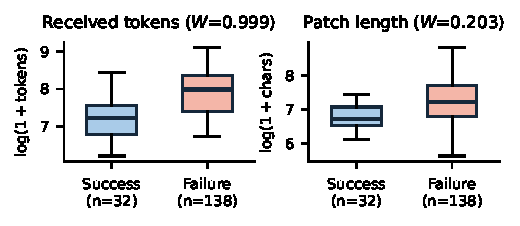
\includegraphics[width=\columnwidth]{figures/v2/eda.pdf}
\caption{Training-only distributions, log-transformed for display; boxes show quartiles and outliers are omitted.}
\label{fig:eda}\end{figure}

We test \textbf{H1}: dual encoders improve over numeric inputs under the same kNN family; \textbf{H2}: patch information adds value beyond logs; \textbf{H3}: failures contaminating the normal references degrade performance. These exploratory v2 hypotheses follow earlier numeric experiments, not an independent preregistration.

\section{Method}
\paragraph{Six-stage primary pipeline.}
(1) Normalize permitted text. (2) Encode log chunks with frozen \texttt{all-MiniLM-L6-v2}: 224 content tokens, 32 overlap, non-special token mean pooling, equal chunk averaging within steps, then equal step averaging and normalization. (3) Split patch hunks into 480-token chunks with overlap 64, encode with frozen \texttt{codebert-base}, mean-pool non-special tokens, aggregate using recorded chunk weights, and normalize. This gives 384-D log and 768-D patch vectors. Long inputs are chunked rather than silently truncated; mean pooling loses chronology.

(4) Store successful training vectors as references. For two nonempty channels,
\begin{equation}
d(x,r)=\tfrac12\left[\tfrac{1-\cos(l_x,l_r)}2+\tfrac{1-\cos(p_x,p_r)}2\right].
\end{equation}
Both channels empty gives channel distance zero; only one empty gives one. (5) Score by mean distance to $k$ nearest successful references, $k\in\{1,3,5\}$. (6) Use validation to select $k$ and alert threshold, then evaluate outer-test rows. Encoder inference is not fine-tuning; reference construction and calibration are separate learned components.

\paragraph{Tiers and controls.}
T1 scores error rate, $0.1$ times repeated-tool streak, a final-error indicator, and $0.5$ times absence of a reproduction indicator. This v2 heuristic differs from the old two-feature rule. T2 is dual encoder kNN. T3 is L2 logistic regression on normalized, equally weighted concatenated embeddings, with balanced class weights and $C\in\{.01,.1,1,10\}$. The character TF-IDF logistic control uses 3--5-grams, sublinear TF, $\mathrm{min\_df}=2$, at most 20,000 features per channel, and the same $C$ grid. Vocabulary and IDF use only permitted fitting rows.

Numeric controls are normal-only Isolation Forest (200 trees), frozen-ECDF scoring, a numeric AE and supervised XGBoost. The ECDF variant computes smoothed fitting tail probabilities $(1+\#\{r_j\leq x_j\})/(n+1)$ and its upper-tail counterpart, combines negative log tails with fitting skewness, and sums column contributions. Evaluation batches do not alter the fitted reference.

Secondary methods are a 23--16--4--16--23 denoising AE (10\% masking, Huber numeric/BCE binary losses, equal behavior/patch group weights) and a conditional residual predictor fitted on successes: ridge ($\alpha=10$) maps behavior to numeric patch features; logistic ($C=.1$) predicts binary outputs, with Laplace-smoothed constants for one-class targets. Unexpected outputs are not evidence of causal anomalies or intent.

\section{Experimental Setup}
All methods share five stratified outer folds (seed 42). Inner validation uses seed $100+f$, giving approximately 60/20/20\% fitting/validation/test per iteration, with about 32 successful fitting and ten successful validation rows. Each issue has one outer-test prediction; all its chunks stay in the same partition. Normal-reference models fit only successful training rows; supervised methods fit mixed training rows. Validation never enters weights or the reference index.

For each candidate, enumerate validation thresholds and infinities, require empirical FPR $\leq20\%$, and maximize recall, breaking ties by balanced accuracy then higher threshold. Select the candidate with greatest resulting validation balanced accuracy, preferring smaller $k/C$ on ties. Freeze model and threshold together, without refitting on validation. This implemented tie rule is explicit. About ten validation successes cannot certify low test FPR. Numeric random models use seeds 42/123/456; deterministic methods run once.

Primary metrics are balanced accuracy (BA), FPR, failure recall, and unflagged success fraction $TN/(TN+FN)$, with raw counts and coverage. Fold-dependent score scales make pooled raw-score AP/AUC potentially misleading; Table~\ref{tab:main} instead gives \emph{mean within-fold AP}. Saved pooled rankings are descriptive, not calibrated cross-fold rankings. We report fold variation separately from seed variation. Paired class-stratified bootstrap intervals use 2,000 resamples of OOF predictions; shared training folds make them conditional evidence.

These data were inspected in earlier drafts. Repartitioning does not create a fresh independent test, so v2 is exploratory. Repositories overlap. An additional leave-repository-group-out diagnostic uses fixed $k=3$ and marks two groups unestimable; it is not the identical selected-$k$ protocol. Original extraction did not pin encoder revisions, limiting exact future redownload reproducibility. The v2 numeric AE (24--16--8--16--24, 100 full-batch Adam epochs, lr .001) also differs from historical v1 settings.

\section{Results}
\begin{table*}[t]\centering\small\setlength{\tabcolsep}{5pt}
\begin{tabular}{@{}lrrrrr@{}}\toprule
Method & BA & FPR & Recall & TN/FP/FN/TP & Fold AP\\\midrule
\csname @@input\endcsname generated/v2_main.tex
\bottomrule\end{tabular}
\caption{Seed-42 OOF operating points over 284 runs. Last column: mean within-fold AP; prevalence baseline approximately 0.810. Success/failure counts are 54/230. Secondary models do not replace T2 after observing results.}
\label{tab:main}\end{table*}
\begin{figure*}[t]\centering
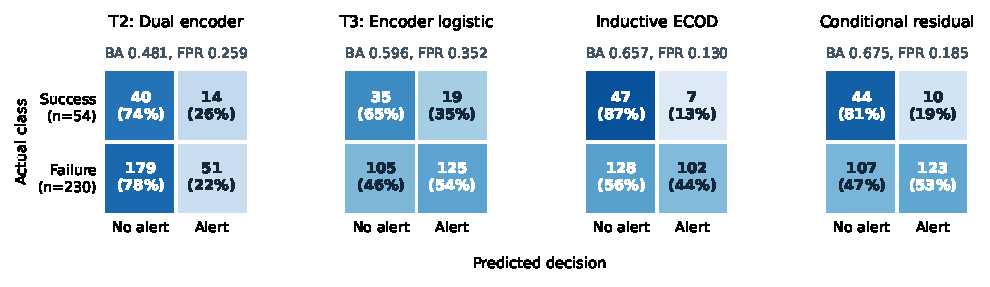
\includegraphics[width=\textwidth]{figures/v2/confusion.pdf}
\caption{Raw OOF confusion counts, colored by fraction within each actual class. T2 leaves 219 runs unflagged, of which only 40 succeed.}
\label{fig:cm}\end{figure*}

\paragraph{Main comparison.}
T2 reaches BA 0.481, FPR 0.259 and recall 0.222. It misses 179/230 failures and falsely flags 14/54 successes (Figure~\ref{fig:cm}). T3 reaches BA 0.596, supervised TF-IDF 0.652, the ECDF variant 0.657, and secondary conditional residuals 0.675. ECDF minus T2 BA is $+0.176$, with conditional paired 95\% interval $[0.114,0.240]$; its FPR difference is $-0.130$ $[-0.241,-0.037]$. These intervals concern the reused data/protocol, not a new deployment population.
\begin{table}[t]\centering\small\setlength{\tabcolsep}{3pt}
\begin{tabular}{@{}lrr@{}}\toprule
Method & Fold BA $\pm$ SD & Seed SD\\\midrule
\csname @@input\endcsname generated/v2_variation.tex
\bottomrule\end{tabular}
\caption{Five-fold variation at seed 42; SD of pooled BA across three optimization seeds. Dash: deterministic method.}
\label{tab:var}\end{table}

\paragraph{Representation and channel ablation.}
Table~\ref{tab:ablation} holds the kNN family and validation policy fixed, although geometry differs: robust Euclidean numeric versus cosine text. Numeric kNN reaches BA 0.641, outperforming all tested encoder variants: H1 is unsupported. Patch-only reaches 0.594 versus log-only 0.456. Adding patches helps logs (H2 narrowly supported), but equal-weight fusion remains worse than patch-only. This implicates the tested pooling/fusion design, not all NLP approaches.
\begin{table}[t]\centering\small
\begin{tabular}{@{}lrrr@{}}\toprule
kNN input & BA & FPR & Recall\\\midrule
\csname @@input\endcsname generated/v2_ablation.tex
\bottomrule\end{tabular}
\caption{Representation/channel comparisons; each $k$ uses the same validation rows.}
\label{tab:ablation}\end{table}

\paragraph{AD-specific contamination.}
Replace $\lfloor np\rfloor$ successful references with training failures, $p\in\{0,.05,.10\}$, keeping reference size and each clean fold's selected $k$ fixed. Nested seeded orders choose removed successes and injected failures. IDs and actual fractions are archived; about 32 references give one/three replacements, not exactly 5/10\%. Both frozen clean cutoffs and validation recalibration are tested. Zero contamination reproduces T2; an earlier mismatched $k=3$ control was corrected before publication. Table~\ref{tab:contam} shows small, nonmonotonic changes, so H3 is unsupported here.
\begin{table}[t]\centering\small
\begin{tabular}{@{}rll@{}}\toprule
Requested \% & Threshold & BA mean $\pm$ SD\\\midrule
\csname @@input\endcsname generated/v2_contamination.tex
\bottomrule\end{tabular}
\caption{Three replacement seeds, fixed-size reference sets and clean model selection.}
\label{tab:contam}\end{table}

\section{Analysis}
\paragraph{Three errors and similarity explanations.}
Cases follow a fixed selection rule on T2 OOF predictions, with full IDs, SHA-256s and excerpts in \texttt{case\_studies.json}. Highest-score FP \texttt{django\_\_django-13230} has $s=.11276$, $\tau=.10865$, margin $+.00411$. Its closest successful reference, \texttt{django-11133}, has log/patch distances .20290/.00655. The log dominates this pair's distance, but a small patch distance does not establish equivalent behavior. The most distant saved step is final \texttt{submit} with a diff observation; this does not establish that long debugging caused the error.

Lowest-score FN \texttt{sympy\_\_sympy-12454} has $s=.02483$, $\tau=.07315$, margin $-.04831$. Its closest reference \texttt{sympy-13647} has distances .04656/.00311. A failed run can resemble successful vectors; similarity alone does not identify its exact semantic defect. Boundary FP \texttt{sympy\_\_sympy-24213} has $s=.07332$, $\tau=.07315$, margin only $+.00018$, illustrating calibration instability.

Pairwise distances explain a nearest reference, while the primary score averages up to five neighbors. The saved step-removal diagnostic holds that one reference fixed instead of rescoring all kNN neighbors. It is a restricted sensitivity check, not additive attribution or causal evidence. This distinction prevents explanations from claiming more than the implementation computed.

\paragraph{Operational interpretation and resources.}
The joint exploratory targets are recall $\geq90\%$, FPR $\leq20\%$, unflagged success fraction $\geq80\%$, and unflagged coverage $\geq5\%$. No method meets them. Only 40/219 (18.3\%) unflagged T2 runs succeed; even conditional residuals leave 151 unflagged with only 44 successes (29.1\%). Reducing review would therefore permit many failed runs to bypass scrutiny. Neither majority-class AP nor higher BA establishes release safety.

The CPU extractor reports 894.8 seconds for all 284 runs (mean 3.14 seconds/run) and peak reported RSS 1191.5 MiB; the downstream runner reports 137.2 seconds and 939.4 MiB. These are aggregate profiler readings, not per-method training times, whole-process-tree peaks or online end-to-end latency. Missing detailed timing limits deployment comparisons. In the fixed-$k$ repository-group diagnostic, BA spans .25--1.0 across ten estimable groups, often with very few successes; this is unstable sensitivity evidence rather than a transfer guarantee.

\section{Conclusion and Limitations}
Frozen text/code embeddings preserve more input content but do not outperform simple numeric controls here. Dual encoder kNN reaches BA 0.481; patch-only improves on it, while a numeric empirical-tail variant reaches 0.657. Contamination has no consistent penalty. All tested methods miss too many failures among unflagged tasks to justify automatic release.

Limitations include one old agent run, few successes, common failures, shared repositories, reused data, unpinned encoder revisions and incomplete correctness labels. Mean pooling removes order, and diff vectors omit requirements and execution semantics. Fresh task-grouped runs and task-conditioned evidence are needed. Keyword masking, task-context encoding and full kNN step-deletion rescoring were not evaluated. We claim no prefix detection, deception diagnosis, unseen-model transfer or production validation.

\section*{Contributions of Each Member}
\begin{itemize}\item \ifdefined\JUDGE Member 1\else Tun-Chieh Yang (315553010)\fi: Pending confirmation.
\item \ifdefined\JUDGE Member 2\else Jia-Cheng Wu (314554059)\fi: Pending confirmation.
\item \ifdefined\JUDGE Member 3\else Min-Quan Wang (315553008)\fi: Pending confirmation.
\item \ifdefined\JUDGE Member 4\else Wei-Chia Chang (315553011)\fi: Pending confirmation.
\item \ifdefined\JUDGE Member 5\else Chun-Ting Hou (315554022)\fi: Pending confirmation.
\end{itemize}
\paragraph{AI Usage Statement.}
Codex assisted protocol design, implementations, local experiments, evidence checks and report/slide drafting. Earlier materials mention Claude/Gemini without confirmed versions or scope. All five member contributions and team verification remain pending confirmation at the user's request; no unconfirmed member work is attributed.
